\documentclass[10pt, aspectratio=169]{beamer}

%======================================================
% Theme (matches Lectures 8/9/10/12)
%======================================================
\usetheme[progressbar=frametitle, sectionpage=progressbar, subsectionpage=progressbar, numbering=fraction, block=fill]{metropolis}

\definecolor{mLightBrown}{HTML}{4D4D4D}
\definecolor{mMediumBrown}{HTML}{2C2C2A}
\definecolor{mDarkBrown}{HTML}{1A1A19}
\definecolor{mDarkTeal}{HTML}{0F6E56}
\definecolor{mDarkRed}{HTML}{B03A2E}
\setbeamercolor{normal text}{fg=mDarkBrown}
\setbeamercolor{alerted text}{fg=mDarkTeal}
\setbeamercolor{frametitle}{bg=mDarkBrown}
\setbeamercolor{progress bar}{fg=mDarkTeal, bg=mDarkTeal!20}

\definecolor{mPaleBg}{HTML}{F4F3EE}
\setbeamercolor{block title}{bg=mDarkBrown!10, fg=mDarkBrown}
\setbeamercolor{block body}{bg=mPaleBg, fg=mDarkBrown}
\newcommand{\hl}[1]{\textcolor{mDarkTeal}{#1}}

%======================================================
\usepackage{amsmath, amssymb, amsthm, mathtools}
\usepackage{cancel}
\usepackage{bm}
\usepackage{booktabs}
\usepackage{array}
\usepackage{xcolor}
\usepackage{colortbl}
\usepackage{multirow}
\usepackage{tikz}
\usetikzlibrary{positioning,arrows.meta,calc,fit,shapes.geometric,decorations.pathmorphing}

%======================================================
\newcommand{\paper}[1]{\textcolor{mLightBrown}{\small\textit{(#1)}}}

% --- the recurring four-question strip ---------------
\newcommand{\qcur}{0}
\newcommand{\qnode}[4]{%
\ifnum#4=\qcur
 \node[draw=mDarkTeal, fill=mDarkTeal!12, thick, rounded corners=1pt, minimum width=3.0cm, minimum height=0.52cm, font=\tiny\bfseries, text=mDarkBrown] (#2) at (#1,0) {#3};%
\else
 \node[draw=mLightBrown!45, rounded corners=1pt, minimum width=3.0cm, minimum height=0.52cm, font=\tiny, text=mLightBrown] (#2) at (#1,0) {#3};%
\fi}
\newcommand{\qstrip}[1]{\renewcommand{\qcur}{#1}%
\begin{center}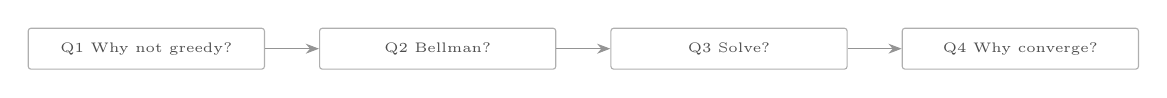
\begin{tikzpicture}
\qnode{0}{q1}{Q1 Why not greedy?}{1}
\qnode{3.7}{q2}{Q2 Bellman?}{2}
\qnode{7.4}{q3}{Q3 Solve?}{3}
\qnode{11.1}{q4}{Q4 Why converge?}{4}
\draw[-{Stealth}, mLightBrown!60] (q1.east) -- (q2.west);
\draw[-{Stealth}, mLightBrown!60] (q2.east) -- (q3.west);
\draw[-{Stealth}, mLightBrown!60] (q3.east) -- (q4.west);
\end{tikzpicture}\end{center}}

%======================================================
\title{Markov Decision Processes \& Dynamic Programming}
\subtitle{A good plan stays good from wherever you land}
\author{Jinkyoo Park}
\institute{KAIST}
\date{\textit{Lecture 7 --- The OR / dynamic-programming origin of sequential decision-making}}

%======================================================
\begin{document}
%======================================================

\maketitle

%==========================================================
\section{The handoff --- from a single choice to a sequence}
%==========================================================

\begin{frame}{Where we are --- the first of two dynamic traditions}
\vspace{2pt}
\begin{center}\footnotesize
\renewcommand{\arraystretch}{1.35}
\begin{tabular}{r|c|c}
 & \textbf{OR / Dynamic Programming} & \textbf{Control Theory} \\
\hline
\textbf{Model-based (origin)}  & \cellcolor{mDarkTeal!20}\textbf{MDP \& DP} \scriptsize(\alert{Lec.\ 7}) & Optimal Control \scriptsize(Lec.\ 9)\\
\hline
\textbf{Data-driven (extension)} & Value-Based RL \scriptsize(Lec.\ 8) & Policy-Based RL \scriptsize(Lec.\ 10)\\
\end{tabular}
\end{center}
\smallskip

This lecture is the \alert{top-left cell}: the operations-research origin of dynamic decision-making. Everything in Lecture 8 (value-based RL) is \emph{this lecture with the model deleted}. The course's other parent --- control theory --- enters in Lecture 9.
\smallskip

\pause
Lecture 1 handed us a single decision over a fixed objective: $\min_x f(x)$. Now decisions arrive \alert{in sequence}, and each one \alert{reshapes the world the next one faces}.
\medskip

\pause
\begin{center}\large
The single optimization splits into time --- and that changes everything.
\end{center}
\end{frame}

\begin{frame}{Why a sequence is not just many single choices}
The fixed point of this lecture, in one line:
\begin{center}\large
\alert{A good plan is one that stays good from wherever you end up.}
\end{center}
\medskip

\pause
A myopic, one-step-greedy choice fails because actions are \alert{coupled through the state}:
\begin{itemize}\setlength\itemsep{2pt}
\item the action you take today changes the state --- and therefore the \emph{options and rewards} available tomorrow;
\item a move that looks best now (high immediate reward) can strand you in a state with no good future;
\item so each decision must be valued not by its immediate payoff, but by \alert{the whole future it unlocks}.
\end{itemize}
\medskip

\pause
This forces a new object. Instead of a number $f(x)$, we need a \alert{value of being in a state} --- the total future reward a good plan can extract from it. And we need an equation that ties each state's value to its successors'. That equation is Bellman's, and it is the whole lecture.
\end{frame}

\begin{frame}{The translation table --- Lecture 1 made dynamic}
Every object of static optimization gains a time index and a successor.
\medskip
\begin{center}\scriptsize\renewcommand{\arraystretch}{1.55}
\begin{tabular}{l|l|l}
\textbf{Lecture 1 (static)} & \textbf{Lecture 7 (dynamic)} & \textbf{What time adds} \\
\hline
decision variable $x$ & action $a_t$ at each state $s_t$ & a choice, repeated \\
objective $f(x)$ & return $\sum_t \gamma^t r_{t+1}$ & rewards accumulate \\
the world is fixed & state evolves $s_{t+1}\sim P(\cdot\mid s_t,a_t)$ & actions reshape the future \\
optimum $x^*$ & optimal \emph{policy} $\pi^*(s)$ & a rule, not a point \\
``what is best here?'' & ``what is best \emph{from here on}?'' & the value function $V^*(s)$ \\
\end{tabular}
\end{center}
\medskip

\pause
The last row is the heart. We stop asking for one best decision and start asking for a \alert{rule} $\pi^*(s)$ that prescribes the best action at \emph{every} state --- precisely because we cannot know in advance which states the future will hand us.
\end{frame}

\begin{frame}{The roadmap --- four questions}
One question per Act. This strip returns at every transition.
\qstrip{0}
\medskip
\begin{itemize}\setlength\itemsep{3pt}
\item \textbf{Q1 --- Why can't we just be greedy?} Actions couple through the state; we need the \alert{value function}.
\item \textbf{Q2 --- What must the value satisfy?} The \alert{Bellman equation} --- recursive consistency, then optimality.
\item \textbf{Q3 --- How do we solve it (given the model)?} \alert{Policy iteration} and \alert{value iteration}.
\item \textbf{Q4 --- Why do both converge?} \alert{Generalized policy iteration} and the contraction that guarantees a unique answer.
\end{itemize}
\end{frame}

%==========================================================
\section{Act 1 --- the arena and the value of a state}
%==========================================================

\begin{frame}{The arena --- a Markov Decision Process}
\qstrip{1}
\medskip
A model of sequential decisions under uncertainty, $\langle \mathcal{S}, \mathcal{A}, T, R, \gamma\rangle$:
\begin{itemize}\setlength\itemsep{2pt}
\item states $\mathcal{S}$ and actions $\mathcal{A}$;
\item transition model $T(s,a,s') = P(s'\mid s,a)$ --- \hl{the dynamics, assumed known};
\item reward $R(s,a,s')$ and discount $\gamma\in[0,1)$;
\item a \alert{policy} $\pi(s)$ mapping each state to an action.
\end{itemize}
\medskip

\pause
\textbf{Markov property:} the next state depends only on the current state and action --- the past is irrelevant given the present. This is what makes a \emph{state-indexed value} well-defined: where you are is a sufficient summary of where you can go.
\medskip

\pause
{\footnotesize\textcolor{mLightBrown}{This is the multi-stage generalization of Lecture 3's decision network: a chance/decision/utility structure, unrolled over time. The known $T,R$ are the assumption Lecture 8 will drop.}}
\end{frame}

\begin{frame}{The value of a state --- counting the whole future}
The \alert{return} from time $t$ is the discounted sum of future rewards $G_t = \sum_{k\ge0}\gamma^k r_{t+k+1}$. The \alert{value} of a state under policy $\pi$ is its expected return:
\[
V^\pi(s) = \mathbb{E}_\pi\big[\,G_t \mid s_t = s\,\big], \qquad
Q^\pi(s,a) = \mathbb{E}_\pi\big[\,G_t \mid s_t=s, a_t=a\,\big].
\]
\medskip
\begin{itemize}\setlength\itemsep{2pt}
\item $V^\pi(s)$ --- how good is it to \emph{be} in $s$ and follow $\pi$ thereafter.
\item $Q^\pi(s,a)$ --- how good is it to \emph{take} $a$ in $s$, then follow $\pi$.
\item $\gamma$ trades immediate vs.\ distant reward, and keeps the infinite sum finite.
\end{itemize}
\medskip

\pause
The value is exactly the object the myopic view lacked: it scores a state by \emph{the entire future a policy can extract}, not by one step's reward. Now we need the equation it must obey.
\end{frame}

%==========================================================
\section{Act 2 --- the Bellman equation}
%==========================================================

\begin{frame}{The Bellman equation --- value, written recursively}
\qstrip{2}
\medskip
Split the return into ``one step now'' plus ``everything after,'' and the Markov property closes the loop:
\[
V^\pi(s) = \sum_{s'} T(s,\pi(s),s')\Big[\,R(s,\pi(s),s') + \gamma\, V^\pi(s')\,\Big].
\]
\medskip
\begin{center}\large
The value of a state $=$ expected immediate reward $+$ discounted value of where you land.
\end{center}
\medskip

\pause
This is the \alert{Bellman expectation equation}: a consistency condition a fixed policy's value \emph{must} satisfy. For finite $\mathcal{S}$ it is a linear system in $\{V^\pi(s)\}$ --- one equation per state, solvable in principle. It turns ``sum an infinite future'' into ``relate each state to its neighbors.''
\end{frame}

\begin{frame}{Bellman optimality --- the principle that makes planning possible}
For the \emph{best} policy, the recursion takes a $\max$:
\[
V^*(s) = \max_{a}\sum_{s'} T(s,a,s')\big[R(s,a,s') + \gamma V^*(s')\big], \quad
Q^*(s,a) = \sum_{s'} T(s,a,s')\big[R + \gamma \max_{a'} Q^*(s',a')\big].
\]
\medskip

\pause
\begin{block}{Bellman's principle of optimality}
\centering
An optimal policy has the property that, whatever the first action and resulting state, the \alert{remaining decisions must themselves be optimal} from that state.
\end{block}
\medskip

\pause
This is the formal version of the lecture's thesis: \emph{a good plan stays good from wherever you land.} It is what lets us solve a daunting sequential problem \alert{one state at a time} --- the optimal long-term choice is the greedy choice with respect to $V^*$. The optimal policy reads straight off:
\[
\pi^*(s) = \arg\max_a \sum_{s'} T(s,a,s')\big[R + \gamma V^*(s')\big].
\]
\end{frame}

%==========================================================
\section{Act 3 --- solving it with the model}
%==========================================================

\begin{frame}{Two halves of one machine --- evaluate, then improve}
\qstrip{3}
\medskip
The Bellman equations are conditions, not algorithms. Dynamic programming turns them into iteration --- two operations:
\medskip
\begin{itemize}\setlength\itemsep{3pt}
\item \textbf{Policy evaluation} --- given $\pi$, compute $V^\pi$ by sweeping the expectation backup to convergence:
\[
V_{k+1}(s) \leftarrow \sum_{s'} T(s,\pi(s),s')\big[R + \gamma V_k(s')\big].
\]
\item \textbf{Policy improvement} --- make $\pi$ greedy with respect to the value just computed:
\[
\pi'(s) = \arg\max_a \sum_{s'} T(s,a,s')\big[R + \gamma V^\pi(s')\big].
\]
\end{itemize}
\medskip

\pause
Improvement is guaranteed never to hurt: $V^{\pi'}\ge V^\pi$, with equality only at the optimum. Alternate the two and you climb to $\pi^*$.
\end{frame}

\begin{frame}{Policy iteration vs.\ value iteration --- two schedules}
\begin{center}\footnotesize\renewcommand{\arraystretch}{1.4}
\begin{tabular}{l|l}
\textbf{Policy Iteration} & \textbf{Value Iteration} \\
\hline
evaluate $\pi$ \emph{to convergence}, then improve & one max-backup per state, repeat \\
$\pi_0 \xrightarrow{\text{PE}} V^{\pi_0} \xrightarrow{\text{PI}} \pi_1 \to \cdots$ & $V_{k+1}(s)\leftarrow \max_a\sum_{s'}T[R+\gamma V_k(s')]$ \\
few, expensive iterations & many, cheap iterations \\
exact policy each round & policy read off only at the end \\
\end{tabular}
\end{center}
\medskip

\pause
Value iteration is just the \alert{Bellman optimality equation turned into an assignment} --- fold evaluation and improvement into a single $\max$-backup. Policy iteration separates them. Both reach the same $V^*,\pi^*$.
\medskip

\pause
{\footnotesize\textcolor{mLightBrown}{Keep value iteration's update in view: $V(s)\leftarrow\max_a\sum_{s'}T[R+\gamma V(s')]$. Lecture 8's Q-learning is \emph{exactly this line} with the model-weighted sum replaced by a single sampled successor.}}
\end{frame}

\begin{frame}{The gridworld --- watching the value propagate}
Iterating the backup, value flows outward from the goal; the greedy policy sharpens into the optimal one.
\medskip
\begin{center}
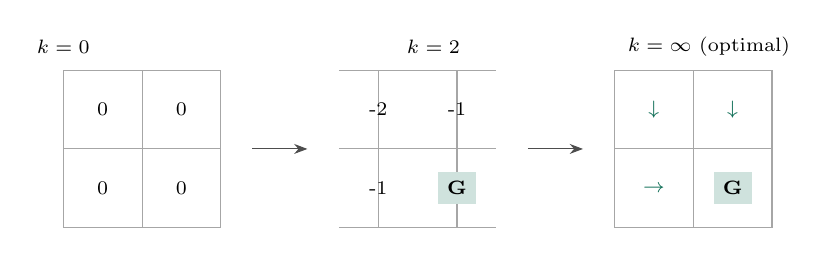
\begin{tikzpicture}[font=\scriptsize]
% k=0
\node at (0,2.3) {$k=0$};
\draw[mLightBrown!50] (0,0) grid (2,2);
\foreach \x in {0,1} \foreach \y in {0,1} \node at (\x+0.5,\y+0.5) {0};
% arrow
\draw[-{Stealth}, mLightBrown] (2.4,1) -- (3.1,1);
% k=1
\node at (4.7,2.3) {$k=2$};
\draw[mLightBrown!50] (3.5,0) grid (5.5,2);
\node at (4.0,1.5){-2}; \node at (5.0,1.5){-1}; \node at (4.0,0.5){-1}; \node[fill=mDarkTeal!20]at (5.0,0.5){\textbf{G}};
\draw[-{Stealth}, mLightBrown] (5.9,1) -- (6.6,1);
% k=inf with policy
\node at (8.2,2.3) {$k=\infty$ (optimal)};
\draw[mLightBrown!50] (7,0) grid (9,2);
\node[mDarkTeal]at (7.5,1.5){$\downarrow$}; \node[mDarkTeal]at (8.5,1.5){$\downarrow$};
\node[mDarkTeal]at (7.5,0.5){$\rightarrow$}; \node[fill=mDarkTeal!20]at (8.5,0.5){\textbf{G}};
\end{tikzpicture}
\end{center}
\medskip

\pause
Each sweep pushes information one step further from the goal. The Markov structure means a state only ever needs to consult its immediate successors --- so a global plan emerges from \alert{purely local backups}. That locality is the gift of the Bellman equation.
\end{frame}

%==========================================================
\section{Act 4 --- why it works}
%==========================================================

\begin{frame}{Generalized Policy Iteration --- the dance behind both}
\qstrip{4}
\medskip
Policy and value chase each other; neither is ever fully consistent with the other until the end.
\medskip
\begin{center}
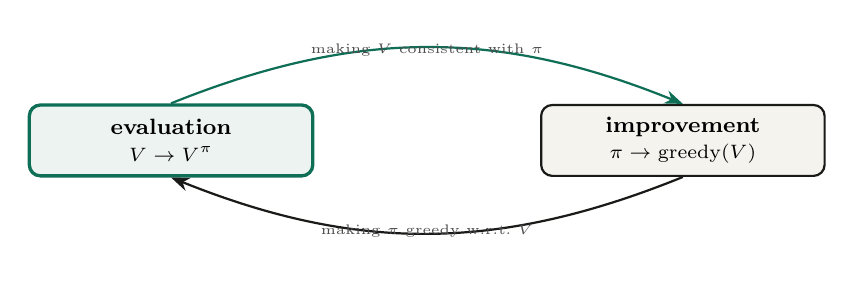
\begin{tikzpicture}[font=\footnotesize]
\node[draw=mDarkTeal, very thick, fill=mDarkTeal!8, rounded corners, minimum width=3.6cm, minimum height=0.9cm, align=center] (eval) at (0,0) {\textbf{evaluation}\\ \scriptsize $V \to V^\pi$};
\node[draw=mDarkBrown, thick, fill=mPaleBg, rounded corners, minimum width=3.6cm, minimum height=0.9cm, align=center] (impr) at (6.5,0) {\textbf{improvement}\\ \scriptsize $\pi \to \text{greedy}(V)$};
\draw[-{Stealth}, mDarkTeal, thick] (eval.north) to[bend left=22] (impr.north);
\draw[-{Stealth}, mDarkBrown, thick] (impr.south) to[bend left=22] (eval.south);
\node[mLightBrown, font=\tiny] at (3.25,1.15) {making $V$ consistent with $\pi$};
\node[mLightBrown, font=\tiny] at (3.25,-1.15) {making $\pi$ greedy w.r.t.\ $V$};
\end{tikzpicture}
\end{center}
\medskip

\pause
Making $\pi$ greedy makes $V$ wrong for the new $\pi$; re-evaluating makes $\pi$ no longer greedy. Yet the two forces have a \alert{single joint fixed point} --- and it is exactly the solution of the Bellman optimality equation. Policy iteration and value iteration are just two \emph{schedules} of this same dance.
\end{frame}

\begin{frame}{Why the fixed point is unique --- the contraction}
The Bellman optimality operator
\[
(\mathcal{T}V)(s) = \max_a \sum_{s'} T(s,a,s')\big[R(s,a,s') + \gamma V(s')\big]
\]
is a \alert{$\gamma$-contraction} in the sup-norm: $\|\mathcal{T}V - \mathcal{T}V'\|_\infty \le \gamma \|V - V'\|_\infty$.
\medskip

\pause
By the Banach fixed-point theorem this gives, for $\gamma<1$, three guarantees at once:
\begin{itemize}\setlength\itemsep{1pt}
\item a \alert{unique} fixed point $V^*$ --- the problem has one answer;
\item value iteration \alert{converges to it from any start}, geometrically at rate $\gamma$;
\item the error contracts every sweep --- $\gamma$ is literally the convergence rate.
\end{itemize}
\medskip

\pause
\begin{center}\large
The discount $\gamma$ is not a modelling afterthought --- it is what makes the whole machine \alert{well-posed}.
\end{center}
This same contraction, applied to \emph{sampled} backups, is what will make Q-learning converge in Lecture 8.
\end{frame}

%==========================================================
\section{Closing}
%==========================================================

\begin{frame}{Where we are --- one parent established}
\vspace{2pt}
\begin{center}\footnotesize
\renewcommand{\arraystretch}{1.35}
\begin{tabular}{r|c|c}
 & \textbf{OR / Dynamic Programming} & \textbf{Control Theory} \\
\hline
\textbf{Model-based} & \cellcolor{mDarkTeal!15}\textbf{MDP \& DP} \;{\scriptsize Lec.\ 7 \checkmark} & Optimal Control \;{\scriptsize Lec.\ 9}\\
\hline
\textbf{Data-driven} & Value-Based RL \;{\scriptsize Lec.\ 8 $\to$} & Policy-Based RL \;{\scriptsize Lec.\ 10}\\
\end{tabular}
\end{center}
\medskip

\pause
We hold the Bellman equation and two exact solvers --- but everything leaned on \alert{knowing $T$ and $R$}. Two roads lead out:
\begin{itemize}\setlength\itemsep{1pt}
\item \textbf{down} (Lecture 8): keep the equation, \alert{delete the model}, learn from samples $\Rightarrow$ value-based RL.
\item \textbf{right} (Lecture 9): the \emph{other} tradition --- control theory --- solving the same dynamic problem in continuous time.
\end{itemize}
\end{frame}

\begin{frame}{Closing --- the one sentence}
\vfill
\begin{center}\large
A sequence of decisions seemed to need a plan for every possible future.\\[8pt]
Bellman showed it needs only a \alert{value for every state} ---\\[4pt]
because an optimal plan, by its nature,\\[4pt]
stays optimal from wherever you happen to land.
\end{center}
\vfill
\pause
\footnotesize
That single insight --- value, defined recursively --- turns an intractable search over plans into local backups over states. It is the foundation of operations-research decision-making, and the equation Lecture 8 will keep even after it throws the model away.
\end{frame}

\begin{frame}[standout]
Questions?
\end{frame}

%==========================================================
\appendix
%==========================================================

\begin{frame}{Backup 1 --- the Bellman equation, derived}
\footnotesize
Start from the definition and peel off one step, using linearity of expectation and the Markov property:
\begin{align*}
V^\pi(s) &= \mathbb{E}_\pi\Big[\textstyle\sum_{k\ge0}\gamma^k r_{t+k+1}\,\Big|\, s_t=s\Big]
= \mathbb{E}_\pi\Big[r_{t+1} + \gamma\textstyle\sum_{k\ge0}\gamma^k r_{t+k+2}\,\Big|\, s_t=s\Big]\\
&= \sum_{s'} T(s,\pi(s),s')\Big[R(s,\pi(s),s') + \gamma\,\mathbb{E}_\pi\big[\textstyle\sum_{k\ge0}\gamma^k r_{t+k+2}\mid s_{t+1}=s'\big]\Big]\\
&= \sum_{s'} T(s,\pi(s),s')\Big[R(s,\pi(s),s') + \gamma\, V^\pi(s')\Big]. \qquad\blacksquare
\end{align*}
\medskip
\textbf{Optimality form.} Maximizing over the first action and noting that the remainder must be optimal (principle of optimality) replaces $\pi(s)$ by $\max_a$ and $V^\pi$ by $V^*$, giving the Bellman optimality equation. The $Q$-form follows by conditioning on $(s,a)$ before the transition.
\end{frame}

\begin{frame}{Backup 2 --- the contraction proof}
\footnotesize
\textbf{Claim.} $\|\mathcal{T}V - \mathcal{T}V'\|_\infty \le \gamma\|V-V'\|_\infty$, where $(\mathcal{T}V)(s)=\max_a\sum_{s'}T(s,a,s')[R+\gamma V(s')]$.
\medskip

For any state $s$, using $|\max_a f(a) - \max_a g(a)| \le \max_a |f(a)-g(a)|$:
\begin{align*}
|(\mathcal{T}V)(s) - (\mathcal{T}V')(s)|
&\le \max_a \Big|\sum_{s'} T(s,a,s')\,\gamma\,[V(s') - V'(s')]\Big|\\
&\le \gamma \max_a \sum_{s'} T(s,a,s')\,|V(s')-V'(s')|
\le \gamma \|V - V'\|_\infty,
\end{align*}
since $\sum_{s'}T(s,a,s')=1$. Taking the max over $s$ gives the claim. \hfill$\blacksquare$
\medskip
\textbf{Consequence (Banach).} For $\gamma<1$, $\mathcal{T}$ has a unique fixed point $V^*$, and $V_{k+1}=\mathcal{T}V_k$ converges to it from any $V_0$ with $\|V_k - V^*\|_\infty \le \gamma^k\|V_0 - V^*\|_\infty$. The same argument with the sampled operator underlies Q-learning's convergence (Lecture 8, Backup 2).
\end{frame}

\begin{frame}{Backup 3 --- policy improvement never hurts}
\footnotesize
\textbf{Policy improvement theorem.} Let $\pi' (s)=\arg\max_a Q^\pi(s,a)$. Then $V^{\pi'}(s)\ge V^\pi(s)$ for all $s$.
\medskip

\textbf{Sketch.} By construction $Q^\pi(s,\pi'(s)) = \max_a Q^\pi(s,a) \ge Q^\pi(s,\pi(s)) = V^\pi(s)$. Now expand $V^\pi(s)\le Q^\pi(s,\pi'(s))$ one step at a time, each time replacing a $\pi$-action by the $\pi'$-action and applying the same inequality to the successor:
\[
V^\pi(s) \le \mathbb{E}_{\pi'}[r_{t+1} + \gamma V^\pi(s_{t+1})] \le \mathbb{E}_{\pi'}[r_{t+1} + \gamma\, Q^\pi(s_{t+1},\pi'(s_{t+1}))] \le \cdots \le V^{\pi'}(s).
\]
\textbf{Why it terminates.} In a finite MDP there are finitely many deterministic policies; each improvement strictly increases value unless $\pi$ is already greedy w.r.t.\ its own value --- which is exactly the Bellman optimality condition. Hence policy iteration reaches $\pi^*$ in finitely many steps.
\end{frame}

\begin{frame}{Backup 4 --- asynchronous and in-place DP}
\footnotesize
The sweeps above updated all states in lockstep. Neither is required.
\medskip

\textbf{In-place value iteration.} Overwrite $V(s)$ immediately and reuse the new value within the same sweep; converges, often faster (it propagates fresh information sooner).
\medskip

\textbf{Asynchronous DP.} Back up states in \emph{any} order, even repeating some and skipping others --- as long as every state is updated infinitely often, convergence to $V^*$ still holds. This decouples computation from a rigid sweep and is what makes DP scale to large or prioritized state sets (e.g.\ prioritized sweeping).
\medskip

\textbf{Why this matters for RL.} Sampled RL is, in effect, \emph{asynchronous DP driven by the states the agent happens to visit}: Q-learning backs up whatever $(s,a)$ the trajectory lands on, in whatever order experience delivers them. The convergence guarantee for asynchronous DP is the model-based ancestor of the ``visit every state infinitely often'' condition in Lecture 8.
\end{frame}

\end{document}
